\chapter{\sf Classical Nucleation Theory}\label{ch:nucleation}


Consider a pure liquid material capable of undergoing phase transition to a crystalline solid state. The atoms of the disordered liquid phase undergo constant thermal fluctuations, occasionally stochastically arranging into a structure resembling a small grain of the crystalline solid. These grains can then proceed to either dissolve back into disordered liquid due to further fluctuations, or continue growing as more atoms attach to the original structure. If the liquid is above its melting temperature, the grains will always eventually dissociate into component liquid atoms. However, below the melting temperature, whether the grains are stable to fluctuations and continue growing or not depends on their size, density, shape, as well as other factors. Classical nucleation theory (CNT) \cite{hoyt_phasetransf,sear07} attempts to predict the rate of appearance of stable solid grains under the simplest possible assumptions for factors determining their stability.

We begin this chapter by presenting the basic assumptions and predictions of CNT, formulated for a two-dimensional system. We then take a short detour to introduce the general Fokker-Planck (FP) equation, which is followed by a description of the specific form of this equation used in CNT. The FP equation then provides an approximate form for the time-dependent nucleation rate predicted by CNT. We conclude with our expectations in applying CNT to nucleation in the PFC model, including problems we will face.




%%%%%%%%%%%%%%%%%%%%%%%%%%%%%%%%%%%%%%%%%%%%%%%%%%%%%%%%%%%%%%%%%%%%%%%%%%%%%%%%%%%%
\section{Work of formation}\label{sec:nuc_work}

In CNT, the interior of a solid grain is treated as consisting of bulk solid, with a sharp interface separating it from the liquid phase around. The `work of formation' $W$ is the free energy required to form such a grain from the original liquid phase. $W$ consists of a bulk term, which represents the difference between the free energies of the solid and liquid phase, as well as a surface term representing the energy penalty for the existence of an interface. We write
%%
\begin{equation}\label{eq:nuc_work}
W = V\Delta G + A\gamma
\end{equation}
%%
where $\Delta G$ is the difference in local free energy density between the initial and final phases, $\gamma$ is the interfacial energy density, $V$ is the volume of the grain and $A$ is its interfacial surface area. $\gamma$ is always of positive sign, as physical systems attempt to minimize the surface area between different phases. If the temperature of the liquid phase is above its melting point, the liquid phase is more favorable than the solid phase, leading to a positive $\Delta G$ and thus a $W$ increasing with grain size. Any grains stochastically appearing would then always dissolve back to liquid as the system relaxes to minimum energy. On the other hand, for a temperature below the melting point, the solid phase is favored, leading to a negative $\Delta G$. As surface area generally scales slower than volume as a grain's size increases, $W$ then exhibits a global maximum. This global maximum defines the nucleation energy barrier: any stochastically-forming grain large enough to surpass the position of the maximum is energetically favored to keep growing, and vice versa for grains that do not surpass the maximum. Figure \ref{fig:nuc_work} sketches $W$ and its two component terms in equation \ref{eq:nuc_work}.

\begin{figure}[h]
    \centering
\subfloat[]
{
    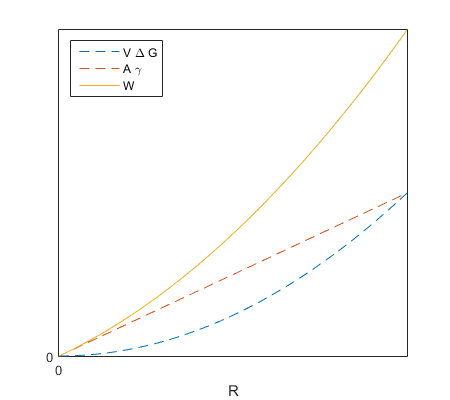
\includegraphics[width=0.5\textwidth]{fig_nuc/nuc_work1}
}
\subfloat[]
{
    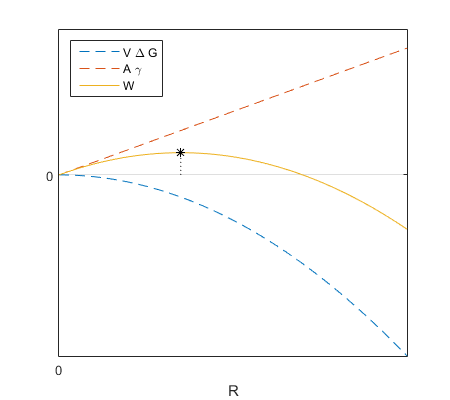
\includegraphics[width=0.5\textwidth]{fig_nuc/nuc_work2}
}
\caption{Sketch of $W$ and its component terms (y-axis) as a function of radius $R$ of the grain, assuming the grain is two-dimensional and circular. Blue is the bulk term, red is the interfacial term, and yellow is the sum $W$. (a) is for temperatures above the freezing point, (b) is for temperatures below the freezing point, also showing the height and position of the nucleation barrier in black.}\label{fig:nuc_work}
\end{figure}

Before continuing, we differentiate between two types of nucleation: homogeneous and heterogeneous. Heterogeneous nucleation occurs in contact with already-present surfaces, such as on the edges of the liquid's container, on earlier-formed solid grains, or on impurities suspended in the liquid. Homogeneous nucleation occurs in the middle of the liquid bulk, independently of position in the bulk (assuming a homogeneous liquid). The nucleation barrier for heterogeneous nucleation is always lower than for homogeneous, due to favorable attractive forces between the nucleating phase and the already-present surfaces \cite{sear07}. However, the number density of possible nucleation sites is much larger for homogeneous nucleation, as it can occur at any point in the liquid. The rate of heterogeneous nucleation is thus much more significant than homogeneous in most materials at small undercooling below the freezing point, where the homogeneous nucleation barrier is too large to realistically observe any homogeneous nucleation events, while homogeneous rate surpasses heterogeneous once sufficient undercooling is achieved. In this work we will concentrate on homogeneous nucleation, as its formulation is simpler and can be easily extended to the heterogeneous case by modifying the form of $W$.

As nature tends to minimize surface area, CNT assumes homogeneous nucleation results in spherical grains. The work of formation in a two-dimensional system can then be written as
%%
\begin{equation}\label{eq:nuc_work_circle}
W(R) = \pi R^2\Delta G + 2\pi R \gamma
\end{equation}
%%
where $R$ is the radius of the grain. The nucleation energy barrier is given by the maximum of equation \ref{eq:nuc_work_circle}, with value $W^*$ and position $R^*$ found to be
%%
\begin{equation}\label{eq:nuc_work_circle_max}
W^* = -\pi\frac{\gamma^2}{\Delta G}, \qquad R^* = -\frac{\gamma}{\Delta G}
\end{equation}
%%
recalling that $\Delta G <0$ below the freezing point. A critical nucleus is then defined to be a grain of radius $R^*$, and larger grains are termed post-critical nuclei.

CNT assumes that atoms in a grain have their mass evenly distributed throughout the grain. We can thus rewrite equation \ref{eq:nuc_work_circle} in terms of the number of atoms in the grain, giving
%%
\begin{equation}\label{eq:nuc_work_g}
W(g) = vg\Delta G + sg^{1/2} \gamma
\end{equation}
%%
where $g$ is the number of atoms, and $v$ and $s$ are the area and interfacial length of a two-dimensional grain consisting of 1 atom ($g=1$) respectively. The critical nucleus' number of atoms $g^*$ is then found similarly as in equation \ref{eq:nuc_work_circle_max}, giving
%%
\begin{equation}\label{eq:nuc_crit_num_g}
g^* = \left(-\frac{s\gamma}{2v\Delta G}\right)^2
\end{equation}
%%

%%%%%%%%%%%%%%%%%%%%%%%%%%%%%%%%%%%%%%%%%%%%%%%%%%%%%%%%%%%%%%%%%%%%%%%%%%%%%%%%%%%%
\section{Steady state rate of nucleation}\label{sec:nuc_steadyrate}

In CNT, each atom in the liquid can aggregate more atoms around it to form a grain, and hence each atom is a possible homogeneous nucleation site. Let $\rho_1$ be the number density of individual atoms in the liquid, equivalently the number density of grains of size $g=1$. If the liquid is allowed to remain at a specific temperature long enough to reach a `steady state', the number density of grains formed due to fluctuations and consisting of $g$ atoms can be written as
%%
\begin{equation}\label{eq:nuc_grainsdist_ss}
\rho(g) = \rho_1 \exp\left(-\frac{W(g)}{k_B T}\right)
\end{equation}
%%
where grains requiring a work of formation of $W(g)$ are assumed to follow the appropriate Boltzmann distribution. Equation \ref{eq:nuc_grainsdist_ss} neglects grains that stabilize and keep growing due to being post-critical after stochastically forming.

CNT predicts the `steady state' rate of homogeneous nucleation per unit volume to be \cite{hoyt_phasetransf}
%%
\begin{equation}\label{eq:nuc_rate_ss}
J_{ss} = Zj^*\rho(g^*)= Zj^* \rho_1\exp\left(-\frac{W^*}{k_B T}\right)
\end{equation}
%%
where $j^*$ is the rate of attachment of atoms to a critical nucleus, and $Z$ is the so-called Zeldovich factor. Multiplying the number density $\rho(g^*)$ of exactly critical nuclei by $j^*$ gives the rate that these critical nuclei become post-critical. The Zeldovich factor is a value less than 1 that accounts for the possibility of fluctuations causing a post-critical nucleus to lose enough atoms to revert to pre-critical, which is known to scale in two dimensional systems as
%%
\begin{equation}\label{eq:nuc_Z_scaling}
Z \propto \left(-\frac{1}{k_B T}\frac{\partial^2 W}{\partial g^2}\Bigr|_{g=g^*}\right)^{1/2} \propto \left(\frac{(g^*)^{-3/2}\gamma}{k_B T}\right)^{1/2} \propto \frac{(-\Delta G)^{3/2}}{\gamma  (k_B T)^{1/2}}
\end{equation}
%%

In general, the exponential factor in equation \ref{eq:nuc_rate_ss} is the most significant in determining the rate of nucleation, though the attachment rate $j^*$ might also be of significant effect depending on the material \cite{hoyt_phasetransf}.

As an aside, the rate of heterogeneous nucleation can be obtained by switching $\rho$ to the number density of heterogeneous nucleation sites (such as impurity particles) and $W^*$ to the appropriate work of formation for a heterogeneous nucleus.

We note that the term `steady state' is misleading, in that it implies the system is at some sort of equilibrium when in fact a liquid capable of phase transition through nucleation is a metastable phase. Rather, `steady state' is to be understood as an assumption that the liquid has been at its current temperature for long enough that nucleation happens at a constant rate. In general, a liquid that starts at a temperature above its freezing point and is then rapidly quenched to below the freezing point will not instantly exhibit this nucleation rate. Instead, a certain amount of time, known as the `incubation' time, must pass before the nucleation rate begins approaching its steady state value. To obtain the time-dependent rate of nucleation, we must define a time-dependent version of the grain number density given in equation \ref{eq:nuc_grainsdist_ss}, as well as a corresponding time-evolution PDE for that density. This PDE is a specific form of the Fokker-Planck (FP) equation, introduced in the following sections.

%%%%%%%%%%%%%%%%%%%%%%%%%%%%%%%%%%%%%%%%%%%%%%%%%%%%%%%%%%%%%%%%%%%%%%%%%%%%%%%%%%%%
\section{The FP equation in general}\label{sec:nuc_fopl_general}

Consider a set of stochastic real scalar variables each corresponding to a point in time, $\{X(t) : t \in \mathbb{R} \}$. This set can represent a stochastic physical process, such as the position of a particle moving in a random direction at any given time. Let $P(X,t)$ be the probability density of $X(t)$, meaning the probability that $a\leq X(t) \leq b$ for some $t$ is
%%
\begin{equation}
\mathrm{Pr}[a\leq X(t) \leq b,t]=\int_a^b P(X,t)dX
\end{equation}
%%

We assume the stochastic process represented by $X(t)$ is a `Markov process': Given the probability density $P(X,t_1)$ at time $t_1$, all future probability densities $P(X,t_2)$ for $t_2>t_1$ can be determined with no knowledge of past probability densities $P(X,t_0)$ for $t_0<t_1$. Heuristically, this can be seen as requiring the process to be deterministic in a specific sense: Despite the variables $X(t)$ not being deterministic themselves, the probability density $P(X,t)$ evolves deterministically through time.

The goal is to obtain the time-evolution PDE for the probability density function $P(X,t)$, though the general derivation \cite{kolpas07,gardiner_stochastic} of this PDE is outside the scope of this work. The full derivation allows a PDE of arbitrary order in $X$, but here we truncate the PDE to 2nd order in $X$, giving
%%
\begin{equation}\label{eq:fopl_general}
\frac{\partial P(X,t)}{\partial t}= \frac{\partial^2}{\partial X^2} (D(X,t)P(X,t)) -  \frac{\partial}{\partial X}(\mu(X,t)P(X,t))
\end{equation}
%%
where the coefficients $D(X,t)$ and $\mu(X,t)$ correspond in many physical systems to the diffusion coefficient and the drift coefficient respectively. This PDE is the general Fokker-Planck equation for a one-dimensional stochastic variable.

The prototypical example utilizing equation \ref{eq:fopl_general} would be Brownian motion of a particle, such as the motion exhibited by a pollen particle suspended in water. Such a particle moves in a random direction at any given point in time as water molecules bump into it. This motion can be modeled as a random walk: Let $X(t)$ be the one-dimensional position at time $t$ of a particle that moves every time interval $\tau$ a distance of $\lambda \pm \epsilon$ with equal probability for either sign. It can be shown \cite{gardiner_stochastic} that, in the limit where $\tau$ is small compared to the total time considered, the probability density $P(X,t)$ of the particle's position evolves according to equation \ref{eq:fopl_general} with constant coefficients $D=\epsilon^2/2\tau$ and $\mu=\lambda/\tau$. Figure \ref{fig:randwalk1} shows the paths taken by a few such particles starting from the same initial position. Figure \ref{fig:randwalk2} shows the corresponding position probability density evolving through time, with the initial position represented by a Dirac $\delta$ function at the starting time. As mentioned above, the FP equation thus allows us to calculate the particle's position probability distribution deterministically, despite the particle's motion being non-deterministic. In the next section, we will similarly determine the probabilistic evolution of a grain of solid in a fluctuating liquid, as atoms randomly attach to and detach from the grain.

\begin{figure}[h]
    \centering
\subfloat[]
{
    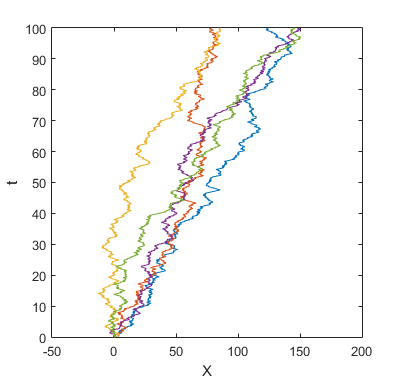
\includegraphics[width=0.5\textwidth]{fig_nuc/randwalk1}
    \label{fig:randwalk1}
}
\subfloat[]
{
    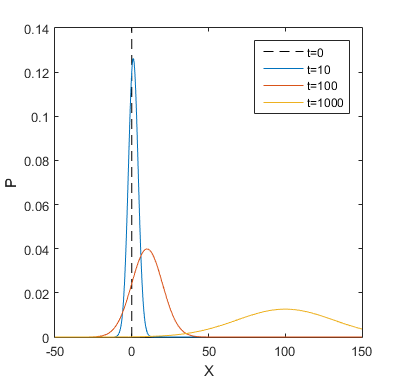
\includegraphics[width=0.5\textwidth]{fig_nuc/randwalk2}
    \label{fig:randwalk2}
}
\caption{(a) The positions $X(t)$ for 5 particles undergoing random walks with $\tau=0.1$, $\lambda=0.1$, $\epsilon=1$, and initial position $X(0)=0$. (b) The probability density for the position of these same particles, at different times.}
\end{figure}

It should be noted that the FP equation for Brownian motion gives the probability distribution for the position of a \textit{single} particle. If we are instead interested in the positions of a large amount of particles present in the same system, we must make the assumption that the particles do not interact with each other as they move. With that assumption, the FP equation can be used for the exact time-evolution of the number density of the Brownian particles. A similar non-interaction requirement proves to be problematic for the application of CNT to the PFC model, as will be discussed in section \ref{sec:nuc_cnt_pfc}.



%%%%%%%%%%%%%%%%%%%%%%%%%%%%%%%%%%%%%%%%%%%%%%%%%%%%%%%%%%%%%%%%%%%%%%%%%%%%%%%%%%%%
\section{The FP equation in CNT}\label{sec:nuc_fopl_nucleation}

Define the time-dependent grain number density in a nucleating liquid phase to be $c(g,t)$, assumed to satisfy $c(g,\infty)=\rho(g)$. Assuming non-interaction between the grains in the liquid, a specific form of the FP equation will give the time-evolution of $c(g,t)$ in the one-dimensional size-space $g$. This FP equation can be derived directly from simple CNT assumptions without the general derivation mentioned in the previous section \cite{hoyt_phasetransf,yoo87,shi90}.

The fluctuations that form grains will now be represented by rates of attachment and detachment of atoms to and from grains. Let $j(g)$ be the rate at which grains of size $g$ grow to $g+1$ by gaining 1 more atom, and conversely $l(g)$ the rate of shrinking from $g$ to $g-1$. The total `flux' of grains in size-space is written as%The specific form of these rates depends on the material under consideration, but in general scales proportionally to the interface length (or area in 3D) of a grain of size $g$. 
%%
\begin{equation}\label{eq:nuc_flux_total}
J(g,t)=j(g)c(g,t)-l(g+1)c(g+1,t)
\end{equation}
%%

At $t=\infty$, the flux must be zero to achieve nucleation steady state. Setting $J(g,\infty)=0$ in equation \ref{eq:nuc_flux_total} gives
%%
\begin{equation}
l(g+1)= \frac{j(g)c(g,\infty)}{c(g+1,\infty)}=\frac{j(g)\rho(g)}{\rho(g+1)}
\end{equation}
%%
which allows rewriting equation \ref{eq:nuc_flux_total} as
%%
\begin{equation}\label{eq:nuc_flux_reduced}
\begin{split}
J(g,t)&=j(g)\left[c(g,t)-\frac{\rho(g)}{\rho(g+1)}c(g+1,t)\right]\\&=j(g)\rho(g)\left[\frac{c(g,t)}{\rho(g)}-\frac{c(g+1,t)}{\rho(g+1)}\right]\\&=-j(g)\rho(g)\frac{\partial}{\partial g}\left[\frac{c(g,t)}{\rho(g)}\right]
\end{split}
\end{equation}
%%
where in the last step the difference was approximated by the appropriate partial derivative.

The growth rate $j(g)$ for a two-dimensional liquid undergoing transition to a crystalline solid is expected to scale as \cite{turnbull49}
%%
\begin{equation}\label{eq:nuc_attachmentrate}
j(g) \propto g^{1/2} k_B T \exp\left(-\frac{\Delta G_A}{k_B T}\right)
\end{equation}
%%
where $\Delta G_A$ is the activation energy needed for an atom to cross the liquid-solid interface to attach to the grain. %For physical systems such as water below its freezing point \cite{jeffery97}, $\Delta G_A$ is estimated to decrease with increasing temperature.

Grains are assumed to all originate as grains of size $g=1$ (i.e. individual atoms). This gives the initial condition of the system to be $c(g,t=0)=\rho_1\delta(g-1)$, recalling that $\rho_1$ is the number of homogeneous nucleation sites available as well as the number density of individual atoms. Grains do not appear or disappear after initial conditions of the system are set, only being allowed to grow and shrink. Conservation of number density in size-space then requires a continuity equation, given as
%%
\begin{equation}\label{eq:nuc_continuity}
\frac{\partial c}{\partial t}=-\frac{\partial J}{\partial g}
\end{equation}
%%

Plugging equation \ref{eq:nuc_continuity} into \ref{eq:nuc_flux_reduced} yields CNT's FP equation, written as
%%
\begin{equation}\label{eq:nuc_fopl}
\frac{\partial c(g,t)}{\partial t}=\frac{\partial}{\partial g}\left[j(g)\rho(g)\frac{\partial}{\partial g}\left(\frac{c(g,t)}{\rho(g)}\right)\right]
\end{equation}
%%

%%%%%%%%%%%%%%%%%%%%%%%%%%%%%%%%%%%%%%%%%%%%%%%%%%%%%%%%%%%%%%%%%%%%%%%%%%%%%%%%%%%%
\section{Analytical approximations for the nucleation rate and incubation time}\label{sec:nuc_fopl_sol}

The time-dependent nucleation rate in the nucleating liquid phase is defined to be the flux in size-space of grains at the critical nucleus size $g^*$, which is $J(g^*,t)$ given by equation \ref{eq:nuc_flux_reduced}. An approximate form for this rate, with the above mentioned initial condition, is obtained by Shi, Seinfeld and Okuyama \cite{shi90} by solving the FP equation \ref{eq:nuc_fopl} using singular perturbation methods. This rate is
%%
\begin{equation}\label{eq:nuc_crit_flux}
J^*(t)=J(g^*,t)=J_{ss} \exp\left[-\exp\left(-2\frac{t}{\tau}+2\lambda\right)\right]
\end{equation}
%%
where we have renamed the rate to $J^*(t)$ for convenience. $J_{ss}$ is the steady state nucleation rate given in equation \ref{eq:nuc_rate_ss}, and $\tau$ and $\lambda$ are values that depend on $g^*$ and determine the incubation time before steady state is achieved. In two dimensions, these are calculated to scale as
%%
\begin{equation}\label{eq:nuc_tau_scaling}
\tau \propto \frac{1}{Z^2 j(g^*)}
\end{equation}
%%
%%
\begin{equation}\label{eq:nuc_lambda_scaling}
\lambda \propto  (g^*)^{-1/2} -1 + \ln\left(Zg^*(1-(g^*)^{-1/2})\right) +\ln\left(2\sqrt{\pi}\right)%O(\ln(g^*))
\end{equation}
%%

It proves to be numerically (and experimentally) easier to calculate the number of post-critical nuclei in a simulated system than it is to directly calculate their rate of appearance. Hence, we derive the time-dependent number density of post-critical nuclei by taking the integral of equation \ref{eq:nuc_crit_flux}. This gives
%%
\begin{equation}\label{eq:nuc_crit_numdens}
I^*(t)=\int_0^t J^*(s)ds=- \frac{J_{ss} \tau}{2} \mathrm{Ei}\left[-\exp\left(-2\frac{t}{\tau}+2\lambda\right)\right]
\end{equation}
%%
where it is implicit that $I^*(t)$ still depends on the critical nucleus size $g^*$, and $\mathrm{Ei}(.)$ is the exponential integral function, defined as
%%
\begin{equation}
\mathrm{Ei}(x)=\int_{-\infty}^x\frac{e^s}{s}ds
\end{equation}
%%

It is not immediately clear from the forms of equations \ref{eq:nuc_crit_flux} and \ref{eq:nuc_crit_numdens} what value should be considered the incubation time, as both $\tau$ and $\lambda$ affect the time needed to reach steady state nucleation rate $J_{ss}$. In this work, we will define the incubation time geometrically, in a manner similar to experimental works such as \cite{legoues84}. As $t \rightarrow \infty$, we calculate that $I^*(t)$ asymptotes to a line given by
%%
\begin{equation}\label{eq:nuc_crit_numdens_asymptote}
I^*(t) \approx J_{ss} ( t - \tau(\lambda+\gamma_{e}/2) )
\end{equation}
%%
where $\gamma_{e}$ is the Euler-Mascheroni constant. The intercept of this line with the horizontal axis is then taken to be the incubation time, written as
%%
\begin{equation}\label{eq:nuc_incubationtime}
t^*=\tau(\lambda+\gamma_{e}/2)
\end{equation}
%%

Figure \ref{fig:nuc_rates_fixedinc} sketches $J^*(t)$ and $I^*(t)$ for a fixed incubation time $t^*$ as $\tau$ and $\lambda$ are varied. We observe that taking $\tau \rightarrow 0$ with $t^*$ fixed leads to $J^*(t)$ approaching a step function of form
%%
\begin{equation}
J^*(t)\approx
\begin{cases}
    J_{ss}& \text{if } t\geq t^*\\
    0              & \text{otherwise}
\end{cases}
\end{equation}
%%

\begin{figure}[h]
    \centering
\subfloat[]
{
    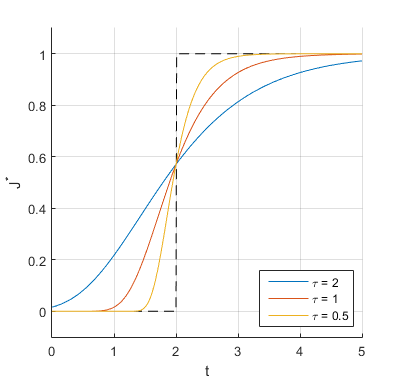
\includegraphics[width=0.5\textwidth]{fig_nuc/nucrates_fixedtinc_J}
}
\subfloat[]
{
    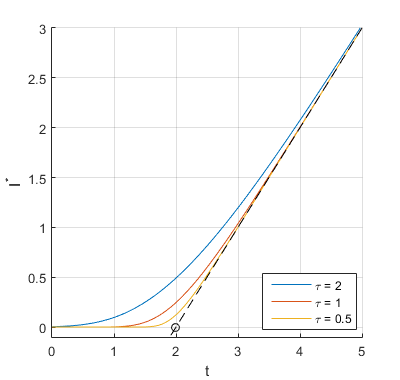
\includegraphics[width=0.5\textwidth]{fig_nuc/nucrates_fixedtinc_I}\label{fig:nuc_rates_fixedinc_b}
}
\caption{(a) Sketch of $J^*(t)$ for $J_{ss}=1$ and $t^*=2$ fixed while $\tau$ varies. Black shows the step function for $\tau \rightarrow 0$. (b) Sketch of $I^*(t)$ for $J_{ss}=1$ and $t^*=2$ fixed while $\tau$ varies. Black shows the asymptote line, and its intersection with the horizontal axis is shown by the black circle.}\label{fig:nuc_rates_fixedinc}
\end{figure}

Finally, we estimate the predicted scalings of $J_{ss}$ and $t^*$ by combining equations \ref{eq:nuc_work_circle_max}, \ref{eq:nuc_crit_num_g}, \ref{eq:nuc_rate_ss}, \ref{eq:nuc_Z_scaling}, \ref{eq:nuc_attachmentrate}, \ref{eq:nuc_tau_scaling}, \ref{eq:nuc_lambda_scaling}, and \ref{eq:nuc_incubationtime}. We find
%%
\begin{equation}\label{eq:nuc_Jss_scaling}
J_{ss} \propto (-\Delta G \, k_B T)^{1/2}\exp\left(-\frac{\Delta G_A}{k_B T}\right)\exp\left(-\frac{\pi}{k_B T}\frac{\gamma^2}{(-\Delta G)}\right)
\end{equation}
%%
%%
\begin{equation}\label{eq:nuc_tinc_scaling}
t^* \propto \left[\frac{1}{(-\Delta G)}+K\frac{\gamma}{(\Delta G)^2}\right]\exp\left(+\frac{\Delta G_A}{k_B T}\right)
\end{equation}
%%
where we have expressed the scalings in terms of the local free energy density difference $\Delta G$ between the solid and liquid phase, the interfacial energy density $\gamma$ of a grain, the temperature factor $k_B T$, and the atomic-attachment activation energy $\Delta G_A$. We also defined
%%
\begin{equation}
K \propto \gamma_e/2-1+ \ln\left(2\sqrt{\pi}\right)+\ln\left(\frac{\gamma}{(-\Delta G \, k_B T)^{1/2}}  \left(1-\frac{(-\Delta G)}{k_B T}\right)  \right) 
%K = \lambda - (g^*)^{-1/2}
\end{equation}
%%
which we will take to be approximately constant due to the slow variation of the logarithmic function. The sign of $K$ depends on the sign of $\lambda$, which in turn can be seen from figure \ref{fig:nuc_rates_fixedinc} and equation \ref{eq:nuc_incubationtime} to depend on how quickly the time-dependent nucleation rate increases from zero to $J_{ss}$.


%%%%%%%%%%%%%%%%%%%%%%%%%%%%%%%%%%%%%%%%%%%%%%%%%%%%%%%%%%%%%%%%%%%%%%%%%%%%%%%%%%%%
\section{Expectations in comparing CNT to nucleation in the PFC model}\label{sec:nuc_cnt_pfc}

To compare nucleation in the PFC model to the predictions of CNT, we will obtain the number density of post-critical nuclei $I^*(t)$ in different simulated PFC systems. This number density will be used to calculate $J_{ss}$ and $t^*$ geometrically as described in the previous section. We will then examine the scaling of these two values in the PFC model and compare them to equations \ref{eq:nuc_Jss_scaling} and \ref{eq:nuc_tinc_scaling}. Chapter \ref{ch:numerics} will detail the numerics used to accomplish these goals, while chapter \ref{ch:results} will showcase the corresponding results. In this section, we preemptively describe the difficulties we expect to encounter due to the assumptions made by CNT in its derivations.

The first difficulty will relate to the finite size of the simulated systems. As CNT assumes grains do not interact and also assumes the number density of single atoms (equivalently, homogeneous nucleation sites) $\rho_1$ is constant through time, its predictions are expected to only hold in early times for the PFC model simulations, before a significant fraction of the liquid phase has transitioned to the solid phase. For this reason, we will be unable to ascertain that the $I^*(t)$ obtained from the simulations has reached its predicted late-time asymptotic value before tapering off due to finite size limits. As such, calculating $J_{ss}$ and $t^*$ geometrically from the presumed asymptote line are only guaranteed to provide lower bounds for these values, rather than exact results.

A second and more subtle difficulty is found in CNT's use of a single variable to describe grains, the number of atoms $g$ in a grain. In both the PFC model and other nucleating systems, this can prove to be an oversimplification, as shape, density, and interface width of the grains can vary independently during the formation process. See for example \cite{lutsko15} where nucleation in globular protein systems is assumed to depend both on interior density and radius of the grains. It is then unclear whether the definitions of $\gamma$ and $\Delta G$ are sound for small pre-critical grains, as $\gamma$ assumes a sharp interface and $\Delta G$ assumes inner grain density equal to the final solid bulk density. In addition, due to vibrational-timescale fluctuations being averaged out in the PFC model, it is unclear whether the assumption of single-atom attachment rate as from equation \ref{eq:nuc_attachmentrate} is a reasonable approximation, and no direct equivalent to the activation energy $\Delta G_A$ is available in this model. Furthermore, as the PFC model's systems consist of a continuous density field rather than discrete atoms, it is feasible that the formation of grains involves fluctuations in the field that do not follow the expected lattice structure at early times, before the grains stabilize. See for example \cite{toth11} where the authors observe what appears to be amorphous structure appearing in the PFC model preceding a crystalline phase, though they are unable to conclude whether this structure represents a separate amorphous phase or very small and tightly packed crystal grains. As part of the discussion of our results, we will attempt to numerically calculate an approximation for the form of the critical nucleus in the PFC model. We will also examine the behavior of the density field during the early formation stage of the grains. These undertakings will be used as guides to whether CNT assumptions are reasonable. We will continue assuming the definitions of $\gamma$ and $\Delta G$ hold, at least in some approximate manner, when examining the scalings of $J_{ss}$ and $t^*$.

The final hurdle relates to the two different temperature parameters that are defined in the PFC model: the effective temperature $\Delta B$ obtained from the parameters in the model's free energy functional in equation \ref{eq:PFC_energyFunctional}, and the fluctuation temperature $T_r$ that follows from the fluctuation-dissipation theorem inherent in defining fluctuations in equation \ref{eq:pfc_noise_dimensionless}. While the authors of \cite{kocher16} effectively couple the values of these two temperature parameters as the other model parameters are varied, there is no definitive way to decide which temperature dependencies of values in the CNT scaling predictions of equations \ref{eq:nuc_Jss_scaling} and \ref{eq:nuc_tinc_scaling} correspond to each of $\Delta B$ and $T_r$. We make the following assumptions related to temperature dependence: Factors of $k_B T$ appearing in the exponential terms $\exp(-\Delta G_A/k_B T)$ and $\exp(-W^*/k_B T)$ are taken to be equivalent to $T_r$, as these exponential terms are based on Boltzmann distribution arguments. We also assume that the temperature dependence of $\Delta G$ is related only to $\Delta B$ and can be approximated from the difference of the local free energy densities of solid and liquid bulks obtained in section \ref{sec:pfc_phasediag}. Further, interfacial energies of stable interfaces in the PFC model are known \cite{provatas_coms} to decrease slowly as $\Delta B$ increases, and we take $\gamma$ to vary as such. Finally, for physical systems such as water below its freezing point \cite{jeffery97}, $\Delta G_A$ is estimated to decrease with increasing temperature. We thus assume that, if its effects are present in the PFC model, $\Delta G_A$ decreases with one or both of the temperature parameters, though its exact dependence is unknown. We will attempt to evaluate these assumptions based on the results we obtain.

%%%%%%%%%%%%%%%%%%%%%%%%%%%%%%%%%%%%%%%%%%%%%%%%%%%%%%%%%%%%%%%%%%%%%%%%%%%%%%%%%%%%
















